\index{I/O access}

The following section describes the low-level mechanism for I/O
access and interrupts on JOP. As JOP is a Java processor no native
functions (usually written in C) are available to access I/O directly
or use C written interrupt handler. We need access to those low-level
functionality from Java for an embedded system. In the following a
hardware abstraction layer (HAL) in Java is proposed, where I/O
devices are mapped to Java objects and interrupt handlers can be
implemented in Java as \code{Runnable}. This section is based on
\cite{jop:hwobj} and \cite{jop:interrupt:handler}.


\section{Hardware Objects}
\label{sec:hwo} \index{hardware object}

Hardware objects map object fields to device registers. Therefore,
field access with bytecodes \code{putfield} and \code{getfield}
accesses device registers. With a correct class that represents a
device, access to it is safe -- it is not possible to read or write
to an arbitrary memory address. A memory area (e.g., a video frame
buffer) represented by an array is protected by Java's array bounds
check. Representing I/O devices as first class objects has following
benefits:

\begin{description}
    \item[Object-oriented:] An object representing a hardware
        device is the most natural integration into an OO
        language
    \item[Safe:] The safety of Java is not compromised. We can
        access only those device registers that are represented
        by the class definition
    \item[Efficient] Device register access is performed by
        single bytecodes \code{getfield} and \code{putfield}. We
        avoid expensive native calls.
\end{description}


\subsection{An Example}
\index{hardware object!example}

Let us consider a simple I/O device, e.g.\ a parallel input/output
(PIO) device -- a common device in embedded systems for control
applications. The PIO provides an interface between I/O registers and
I/O pins. The host captures data on the input pins with a register
read and drives data to the output pins with a register write. The
example PIO contains two registers: the \emph{data register} and the
\emph{control register}. Writing to the data register stores the
value into a register that drives the output pins. Reading from the
data register returns the value that is present at the input pins.

The control register configures the direction for each PIO pin. When
bit $n$ in the control register is set to 1, pin $n$ drives out the
value of bit $n$ of the data register. A 0 at bit $n$ in the control
register configures pin $n$ as input pin. At reset the port is
usually configured as input port -- a safe default
configuration.\footnote{Direction output can result in a short
circuit between the I/O pin and the external device when the logic
levels are different.}

\begin{lstlisting}[float=t,caption={Definition and usage of a parallel port in C},
label=lst:io:c:example]
    typedef struct {
        int data;
        int control;
    } parallel_port;

    #define PORT_ADDRESS 0x10000;

    int inval, outval;
    parallel_port *mypp;
    mypp = (parallel_port *) PORT_ADDRESS;
    ...
    inval = mypp->data;
    mypp->data = outval;
\end{lstlisting}

When the I/O address space is memory mapped, such a parallel port is
represented in C as a structure and a constant for the address. This
definition is part of the board level configuration.
%It is provided by the board manufacturer or for configurable devices,
%such as FPGAs, generated by a system builder (e.g., Altera's
%\emph{SOPC Builder} \cite{quartus} for a NIOS system \cite{NIOS}).
Listing~\ref{lst:io:c:example} shows the parallel port example. The
parallel port is directly accessed via a pointer in C. For a system
with a distinct I/O address space (e.g.\ x86) access to the device
registers is performed via distinct machine instructions. Those
instructions are represented by C functions that take the address as
argument which is not type-safe.

This simple representation of memory mapped I/O devices in C is both
efficient and dangerous. It is efficient as the access via pointers
compiles to simple load and store instructions. It is dangerous as
wrong pointer manipulation can result in erroneous I/O or memory
access. This issue is inherent to C and C programmers are (hopefully)
aware of it. A major aspect that makes Java a safer\footnote{In this
context we consider the safety aspect as safe from programming
errors.} language than C is the avoidance of pointers. A pointer is
in effect an address to data manipulated as data -- an abstraction
that resembles more assembler programming than programming in a
high-level language.

On a standard JVM, native functions, written in C or C++, allow the
low-level access to devices from Java. This approach is not
object-oriented (OO) and incurs a lot of overheads; parameters and
return values have to be converted between Java and C. In an OO
language the most natural way to represent an I/O device is as an
object. Listing~\ref{lst:io:java:example} shows a class definition
for our simple parallel port.

\begin{lstlisting}[float=t,caption={The parallel port device as a simple Java class},
label=lst:io:java:example]
    public final class ParallelPort {
        public volatile int data;
        public volatile int control;
    }

    int inval, outval;
    myport = JVMMagic.getParallelPort();
    ...
    inval = myport.data;
    myport.data = outval;
\end{lstlisting}

The class \code{ParallelPort} is equivalent to the structure
definition for C in Listing~\ref{lst:io:c:example}. Reference
\code{myport} points to the hardware object. The device register
access is similar to the C version. The main difference to the C
structure is that the access requires no pointers. To provide this
convenient representation of I/O devices as objects we just need some
\emph{magic} in the JVM and a mechanism to \emph{create} the device
object and receive a reference to it.


\subsection{Definition}
\index{hardware object!definition}

All hardware classes have to extend the abstract class
\code{HardwareObject} (see Lising~\ref{lst:hwo:marker}). This empty
class serves as type marker. Some implementations use it to
distinguish between plain objects and hardware objects for the field
access. The package visible only constructor disallows creation of
hardware objects by the application code that resides in a different
package.

\begin{lstlisting}[float,caption={The marker class for hardware objects},
label=lst:hwo:marker]

public abstract class HardwareObject {
    HardwareObject() {};
}
\end{lstlisting}


Listing~\ref{lst:hwo:serial} shows a class representing a serial port
with a \code{status} register and a \code{data} register. The status
register contains flags for receive register full and transmit
register empty; the data register is the receive and transmit buffer.
Additionally, we define device specific constants (bit masks for the
\code{status} register) in the class for the serial port. All fields
represent device registers that can change due to activity of the
hardware device. Therefore, they must be declared \code{volatile}.

\begin{lstlisting}[float,caption={A serial port class with device methods},
label=lst:hwo:serial]

public final class SerialPort extends HardwareObject {

    public static final int MASK_TDRE = 1;
    public static final int MASK_RDRF = 2;

    public volatile int status;
    public volatile int data;

    public void init(int baudRate) {...}
    public boolean rxFull() {...}
    public boolean txEmpty() {...}
}
\end{lstlisting}

In this example we have included some convenience methods to access
the hardware object. However, for a clear separation of concerns, the
hardware object represents only the device state (the registers). We
do not add instance fields to represent additional state, i.e.,
mixing device registers with heap elements. We cannot implement a
complete device driver within a hardware object; instead a complete
device driver owns a number of private hardware objects along with
data structures for buffering, and it defines interrupt handlers and
methods for accessing its state from application processes. For
device specific operations, such as initialization of the device,
methods in hardware objects are useful.

\subsection{Access Control}

Usually each device is represented by exactly one hardware object
(see Section~\ref{sec:factory}). However, there might be use cases
where this restriction should be relaxed. Consider a device where
some registers should be accessed by system code only and some other
by application code. In JOP there is such a device: a system device
that contains a 1~MHz counter, a corresponding timer interrupt, and a
watchdog port. The timer interrupt is programmed relative to the
counter and used by the real-time scheduler -- a JVM internal
service. However, access to the counter can be useful for the
application code. Access to the watchdog register is required from
the application level. The watchdog is used for a sign-of-life from
the application. If not triggered every second the complete system is
restarted. For this example it is useful to represent one hardware
device by two \emph{different} classes -- one for system code and one
for application code. We can protect system registers by private
fields in the hardware object for the application.
Listing~\ref{lst:hwo:sys:classes} shows the two class definitions
that represent the same hardware device for system and application
code respectively. Note how we changed the access to the timer
interrupt register to \code{private} for the application hardware
object.

\begin{lstlisting}[float,caption={System and application classes
with visibility protection for a single hardware device},
label=lst:hwo:sys:classes]

public final class SysCounter extends HardwareObject {

    public volatile int counter;
    public volatile int timer;
    public volatile int wd;
}

public final class AppCounter extends HardwareObject {

    public volatile int counter;
    private volatile int timer;
    public volatile int wd;
}
\end{lstlisting}

Another option, shown in Listing~\ref{lst:hwo:sys:setget}, is to
declare all fields private for the application object and use setter
and getter methods. They add an abstraction on top of hardware
objects and use the hardware object to implement their functionality.
Thus we still do not need to invoke native functions.

\begin{lstlisting}[float,caption={System and application classes with setter and getter
methods}, label=lst:hwo:sys:setget]

public final class AppGetterSetter extends HardwareObject {

    private volatile int counter;
    private volatile int timer;
    private volatile int wd;

    public int getCounter() {
        return counter;
    }

    public void setWd(boolean val) {
        wd = val ? 1 : 0;
    }
}
\end{lstlisting}


\subsection{Using Hardware Objects}
\index{hardware object!usage}

Use of hardware objects is straightforward. After obtaining a
reference to the object all that has to be done (or can be done) is
to read from and write to the object fields.
Listing~\ref{lst:hwo:hello:world} shows an example of client code.
The example is a \emph{Hello World} program using low-level access to
a serial port via a hardware object.

\begin{lstlisting}[float=t,caption={A `Hello World' example with low-level device
access via a hardware object},
label=lst:hwo:hello:world]

import com.jopdesign.io.*;

public class Example {

    public static void main(String[] args) {

        BaseBoard fact = BaseBoard.getBaseFactory();
        SerialPort sp = fact.getSerialPort();

        String hello = "Hello World!";

        for (int i=0; i<hello.length(); ++i) {
            // busy wait on transmit buffer empty
            while ((sp.status & SerialPort.MASK_TDRE) == 0)
                ;
            // write a character
            sp.data = hello.charAt(i);
        }
    }
}
\end{lstlisting}


\subsection{Hardware Arrays}
\index{hardware object!arrays}

For devices that use DMA (e.g., video frame buffer, disk, and network
I/O buffers) we map that memory area to Java arrays. Arrays in Java
provide access to raw memory in an elegant way: the access is simple
and safe due to the array bounds checking done by the JVM. Hardware
arrays can be \emph{used} by the JVM to \emph{implement} higher-level
abstractions from the RTSJ such as \code{RawMemory} or scoped memory
\cite{jop:scope:cache}.

\subsection{Garbage Collection}

Interaction between the garbage collector (GC) and hardware objects
needs to be crafted into the JVM. We do not want to \emph{collect}
hardware objects. The hardware object should not be scanned for
references.\footnote{If a hardware coprocessor, represented by a
hardware object, itself manipulates an object on the heap and holds
the only reference to that object it has to be scanned by the GC.}
This is permissible when only primitive types are used in the class
definition for hardware objects -- the GC scans only reference
fields. To avoid collecting hardware objects, we \emph{mark} the
object to be skipped by the GC. The type inheritance from
\code{HardwareObject} can be used as the marker.

For JOP we only define hardware objects with primitive data fields.
Therefore, the hardware objects can be ignored by the GC. The GC
scans only objects where the handles are in the handle area. When the
GC is about to mark and scan an object it first checks if the
reference points into the handle area. If not, the reference is
skipped by the GC. All handles that lie outside of this area are
ignored by the GC. The handles for the hardware objects are allocated
in a special memory area (see Section~\ref{sec:hwo:implementation})
that is ignored by the GC. The same mechanism is already used by the
JVM for some runtime data structures (notable string constants) that
reside in their own memory area.

Handles which are not touched by the GC do not need the additional GC
info fields. We need only two fields: (1) the indirection field and
(2) the class reference or array length field.

\subsection{Hardware Object Creation} \label{sec:factory} \index{hardware object!creation}

The idea to represent each device by a single object or array is
straightforward, the remaining question is: How are those objects
created? An object that represents a device is a typical Singleton
\cite{Go4}. Only a single object should map to one instance of a
device. Therefore, hardware objects cannot be instantiated by a
simple \code{new}: (1) they have to be mapped by some JVM mechanism
to the device registers and (2) each device instance is represented
by a single object.

Each device object is created by its own factory method. The
collection of these methods is the board configuration, which itself
is also a Singleton (the application runs on a single board). The
Singleton property of the configuration is enforced by a class that
contains only static methods. Listing~\ref{lst:hwo:static:fact} shows
an example for such a class. The class \code{IOSystem} represents a
system with three devices: a parallel port, as discussed before to
interact with the environment, and two serial ports: one for program
download and one which is an interface to a GPS receiver.

\begin{lstlisting}[float=t,caption={A factory with static methods for Singleton hardware objects},
label=lst:hwo:static:fact]

package com.board-vendor.io;

public class IOSystem {

    // some JVM mechanism to create the hardware objects
    private static ParallelPort pp = jvmPPCreate();
    private static SerialPort sp = jvmSPCreate(0);
    private static SerialPort gps = jvmSPCreate(1);

    public static ParallelPort getParallelPort() {
        return pp;
    }

    public static SerialPort getSerialPort() {..}
    public static SerialPort getGpsPort() {..}
}
\end{lstlisting}


This approach is simple, but not very flexible. Consider a vendor who
provides boards in slightly different configurations (e.g., with
different number of serial ports). With the above approach each board
requires a different (or additional) \code{IOSystem} class that lists
all devices. A more elegant solution is proposed in the next section.

\subsection{Board Configurations}
\index{hardware object!board configuration}

Replacing the static factory methods by instance methods avoids code
duplication; inheritance then gives configurations. With a factory
object we represent the common subset of I/O devices by a base class
and the variants as subclasses.

However, the factory object itself must still be a Singleton.
Therefore the board specific factory object is created at class
initialization and is retrieved by a static method.
Listing~\ref{lst:hwo:base:fact} shows an example of a base factory
and a derived factory. Note how \code{getBaseFactory()} is used to
get a single instance of the factory. We have applied the idea of a
factory two times: the first factory generates an object that
represents the board configuration. That object is itself a factory
that generates the objects that interface to the hardware device.

\begin{lstlisting}[float=t,caption={A base class of a hardware object
factory}, label=lst:hwo:base:fact]

public class BaseBoard {

    private final static int SERIAL_ADDRESS = ...;
    private SerialPort serial;
    BaseBoard() {
        serial = (SerialPort) jvmHWOCreate(SERIAL_ADDRESS);
    };
    static BaseBoard single = new BaseBoard();
    public static BaseBoard getBaseFactory() {
        return single;
    }
    public SerialPort getSerialPort() { return serial; }

    // here comes the JVM internal mechanism
    Object jvmHWOCreate(int address) {...}
}
\end{lstlisting}

The shown example base factory represents the minimum configuration
with a single serial port for communication (mapped to
\code{System.in} and \code{System.out}) represented by a
\code{SerialPort}. The derived configuration \code{ExtendedBoard}
(listing~\ref{lst:hwo:ext:fact}) contains an additional serial port
for a GPS receiver and a parallel port for external control.

\begin{lstlisting}[float=t,caption={An extended class of a hardware object
factory for a board variation}, label=lst:hwo:ext:fact]

public class ExtendedBoard extends BaseBoard {

    private final static int GPS_ADDRESS = ...;
    private final static int PARALLEL_ADDRESS = ...;
    private SerialPort gps;
    private ParallelPort parallel;
    ExtendedBoard() {
        gps = (SerialPort) jvmHWOCreate(GPS_ADDRESS);
        parallel = (ParallelPort) jvmHWOCreate(PARALLEL_ADDRESS);
    };
    static ExtendedBoard single = new ExtendedBoard();
    public static ExtendedBoard getExtendedFactory() {
        return single;
    }
    public SerialPort getGpsPort() { return gps; }
    public ParallelPort getParallelPort() { return parallel; }
}
\end{lstlisting}



%% MS: we have two different static methods getXXFactory() - could we use one name?
% is this kind of 'overloading' (more hiding) allowed in Java?
% APR its is OK if the signatures are different

Furthermore, we show in those examples a different way to incorporate
the JVM mechanism in the factory: we define well known constants (the
memory addresses of the devices) in the factory and let the native
function \code{jvmHWOCreate()} return the correct device type.

%Figure~\ref{fig:uml} gives a summary example of hardware object
%classes and the corresponding factory classes as a UML class diagram.
%The figure shows that all device classes subclass the abstract class
%\code{HardwareObject}.
%
%\begin{figure}
%    \centering
%    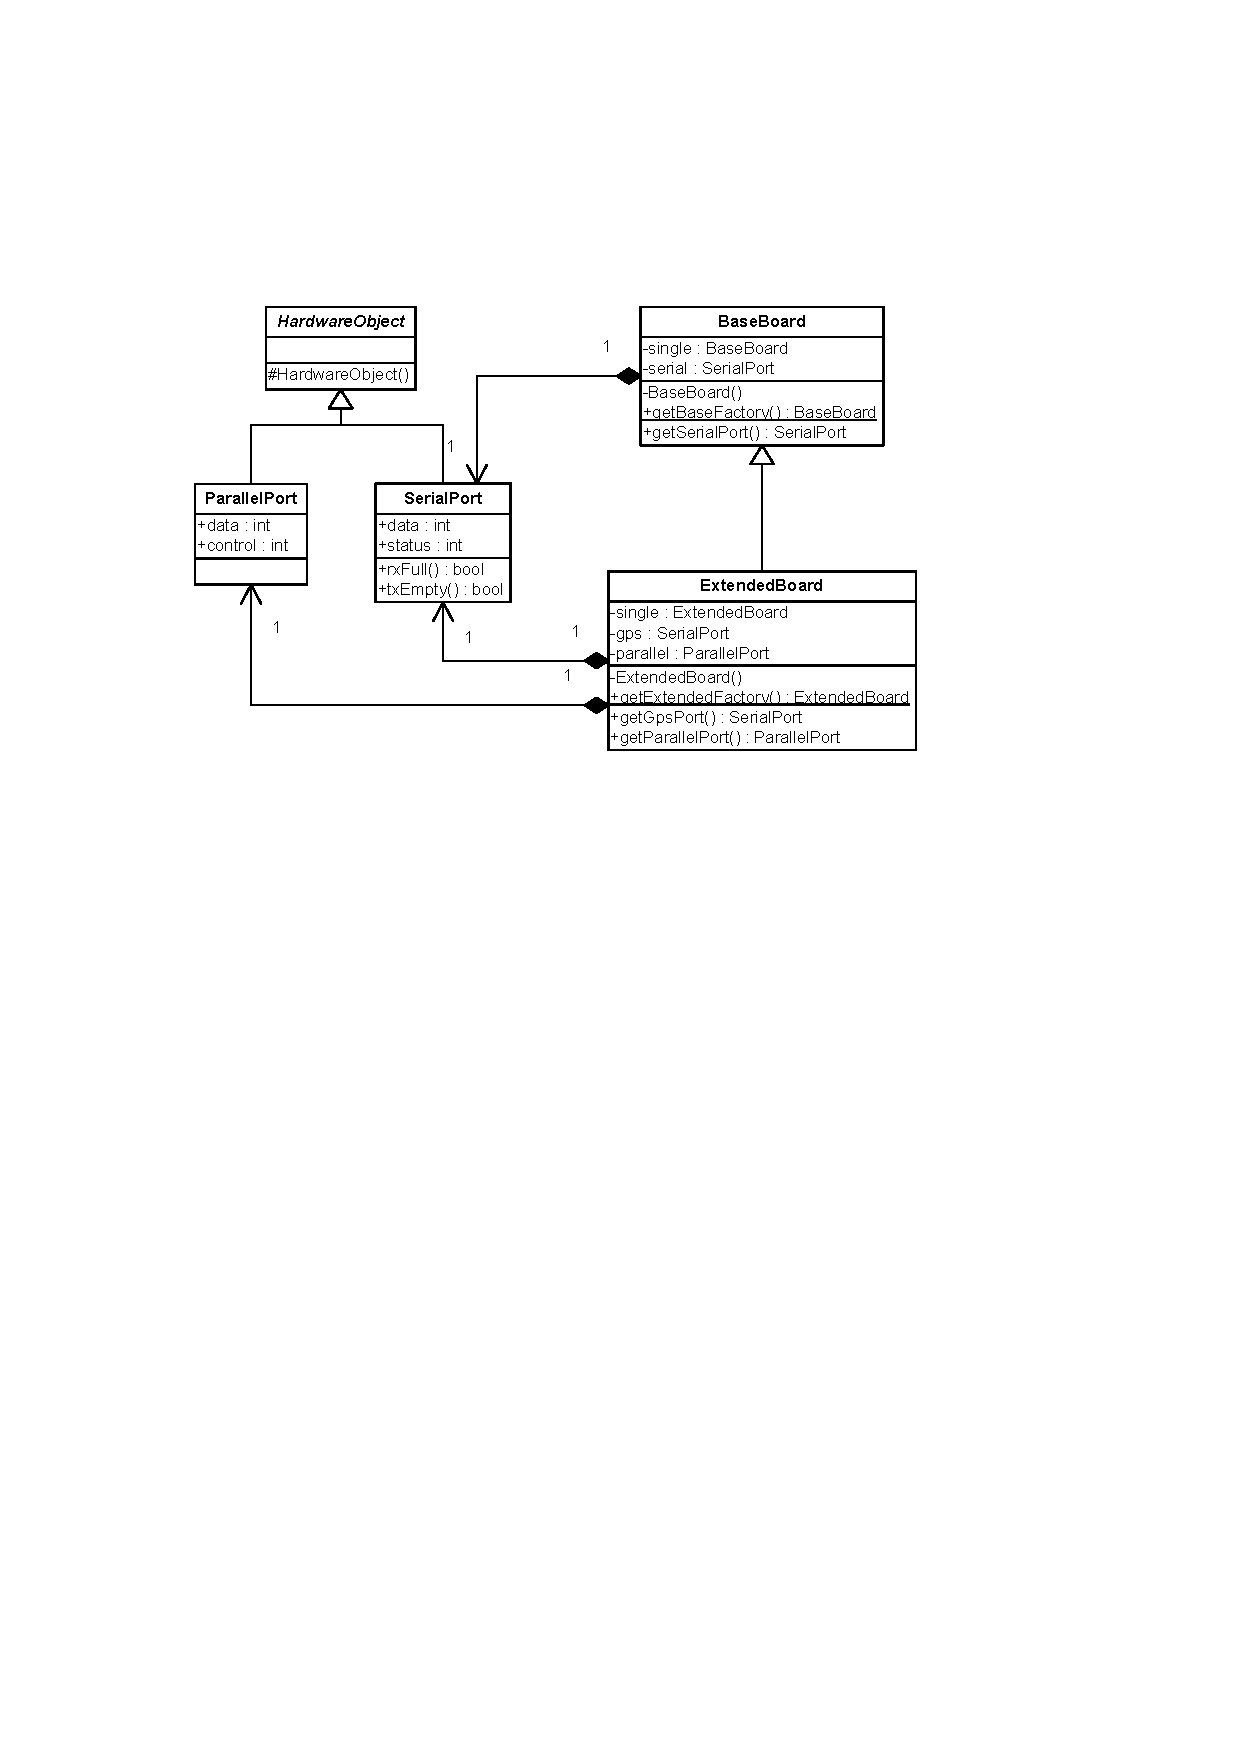
\includegraphics[scale=0.8]{io/uml}
%   \caption{Device object classes and board factory classes}\label{fig:uml}
%\end{figure}
%

\subsection{Implementation}
\label{sec:hwo:implementation} \index{hardware object!implementation}

In this subsection the internals of the hardware object creation are
described. Just to use hardware objects this section can be skipped.
To create new types of hardware objects and the companion factory
this section contains the needed details.

\begin{figure}[t]
    \centering
    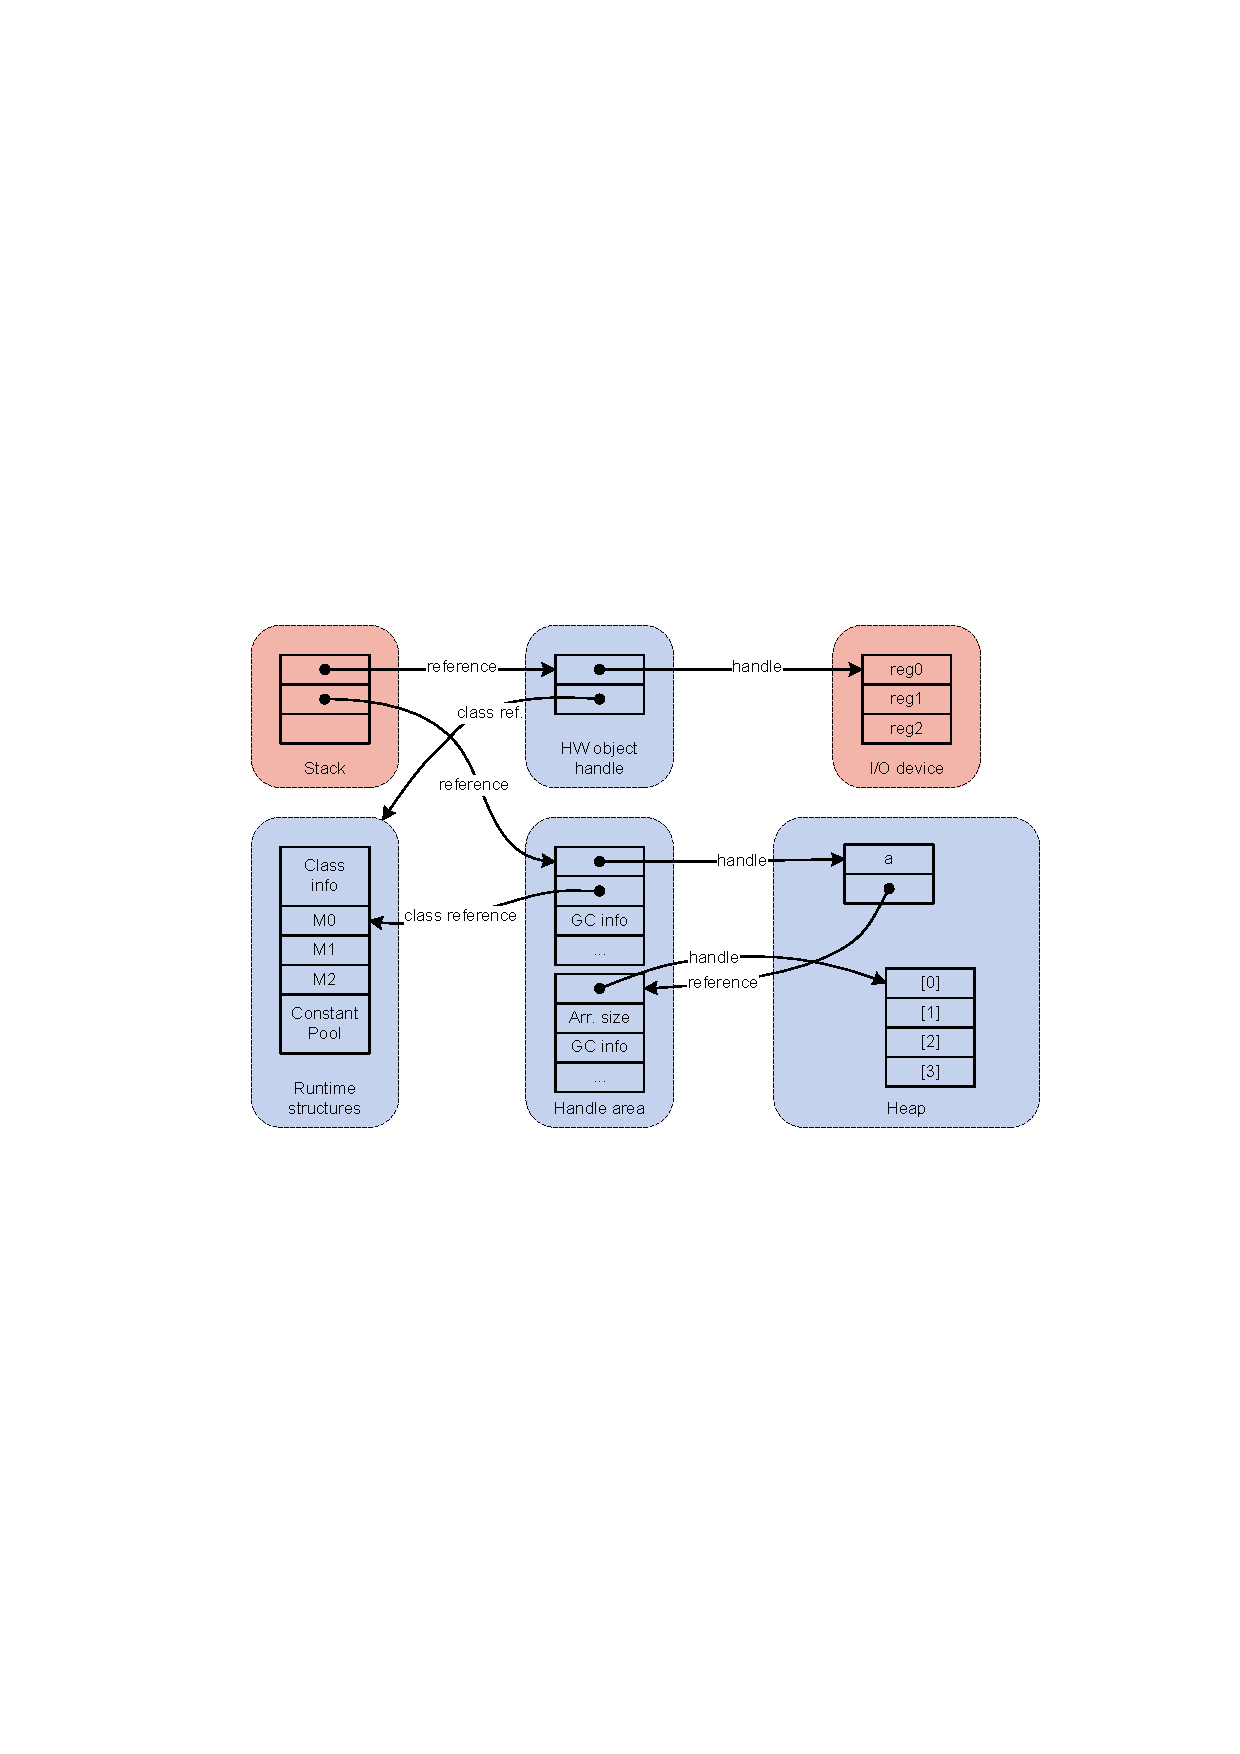
\includegraphics[scale=\picscale]{io/memory}
    \caption{Memory layout of the JOP JVM}\label{fig:hwo:mem}
\end{figure}

In JOP, objects and arrays are referenced through an indirection
called \emph{handle}. This indirection is a lightweight read barrier
for the compacting real-time GC (see Chapter~\ref{chap:rtgc}). All
handles for objects in the heap are located in a distinct memory
region, the handle area. Besides the indirection to the \emph{real}
object the handle contains auxiliary data, such as a reference to the
class information, the array length, and GC related data.
Figure~\ref{fig:hwo:mem} shows an example with a small object that
contains two fields and an integer array of length 4. The object and
the array on the heap just contain the data and no additional hidden
fields. This object layout greatly simplifies our object to device
mapping. We just need a handle where the indirection points to the
memory mapped device registers instead of into the heap. This
configuration is shown in the upper part of Figure~\ref{fig:hwo:mem}.
Note that we do not need the GC information for the hardware object
handles. The factory, which creates the hardware objects, implements
this indirection.

As described in Section~\ref{sec:factory} we do not allow
applications to create hardware objects; the constructor is private
(or package visible).\footnote{For creation of hardware objects with
\codefoot{new} we would need to change the implementation of bytecode
\codefoot{new} to distinguish between normal heap allocated objects
and hardware objects. In the implementation on JOP the hardware
object constructor is package visible to allow the factory to create
a plane object of that type.} Listing~\ref{lst:hwo:jop:base} shows
part of the base hardware object factory that creates the hardware
object \code{SerialPort} and \code{SysDevice}. Two static fields
(\code{SP\_PTR} and \code{SP\_MTAB}) are used to store the handle to
the serial port object. The first field is initialized with the base
address of the I/O device; the second field contains a pointer to the
class information.\footnote{In JOP's JVM the class reference is a
pointer to the method table to speed-up the invoke instruction.
Therefore, the name is \codefoot{XX\_MTAB}.} The address of the
static field \code{SP\_PTR} is returned as the reference to the
serial port object.

\begin{lstlisting}[caption={Simplified version of the JOP base factory},
label=lst:hwo:jop:base]

public class IOFactory {
    private SerialPort sp;
    private SysDevice sys;

    // Handles should be the first static fields!
    private static int SP_PTR;
    private static int SP_MTAB;
    private static int SYS_PTR;
    private static int SYS_MTAB;

    IOFactory() {
        sp = (SerialPort) makeHWObject(new SerialPort(), Const.IO_UART1_BASE, 0);
        sys = (SysDevice) makeHWObject(new SysDevice(), Const.IO_SYS_DEVICE, 1);
    };
    // that has to be overridden by each sub class to get the correct cp
    private static Object makeHWObject(Object o, int address, int idx) {
        int cp = Native.rdIntMem(Const.RAM_CP);
        return JVMHelp.makeHWObject(o, address, idx, cp);
    }
    private static IOFactory single = new IOFactory();
    public static IOFactory getFactory() {
        return single;
    }

    public SerialPort getSerialPort() { return sp; }
    public SysDevice getSysDevice() { return sys; }
}
\end{lstlisting}

The class reference for the hardware object is obtained by creating a
\emph{normal} instance of \code{SerialPort} with \code{new} on the
heap and copying the pointer to the class information. To avoid using
native methods in the factory class we delegate JVM internal work to
a helper class in the JVM system package as shown in
Listing~\ref{lst:hwo:helper}. That helper method returns the address
of the static field \code{SP\_PTR} as reference to the hardware
object. All methods in class \code{Native}, a JOP system class, are
\emph{native}\footnote{There are no \emph{real} native functions in
JOP -- bytecode is the native instruction set. The very few native
methods in class \codefoot{Native} are replaced by special, unused
bytecodes during class linking.} methods for low-level functions --
the code we want to avoid in application code. Method
\code{toInt(Object o)} defeats Java's type safety and returns a
reference as an \code{int}. Method \code{toObject(int addr)} is the
inverse function to map an address to a Java reference. Low-level
memory access methods are used to manipulate the JVM data structures.

\begin{lstlisting}[float,caption={The helper method in the system class \code{JVMHelp} for the hardware object
creation}, label=lst:hwo:helper]

public static Object makeHWObject(Object o, int address, int idx, int
cp) {
    int ref = Native.toInt(o);
    int pcl = Native.rdMem(ref+1);
    int p = Native.rdMem(cp-1);
    p = Native.rdMem(p+1);
    p += idx*2;
    Native.wrMem(address, p);
    Native.wrMem(pcl, p+1);
    return Native.toObject(p);
}
\end{lstlisting}

To disallow the creation with \code{new} in normal application code,
the visibility is set to package. The package visibility of the
hardware object constructor is a minor issue.
%
%% MS: not anymore - code is removed
%The work-around to retrieve the address of a static field from a
%class in Java code is also shown in Listing~\ref{fig:hwobj:helper}.
%%
%% MS: this section contains too much details on JOP.
%% Perhaps remove it.
%%
%
%We want to group all I/O device classes and the Factory classes,
%which describe different boards, in a single package, in our case in
%\code{com.jopdesign.io}. As we have seen in the former section we
%need some native functions in the factory methods. The native
%functions for JOP (class \code{Native}) are located in a system
%package (\code{com.jopdesign.sys}). This system package contains JVM
%internal classes for scheduling, garbage collection, and JVM helper
%methods. As Java does not contain the \emph{friend} construct from
%C++ we have to declare the native functions public -- something we
%wanted to avoid by our hardware objects.
%
%Moving the Factory classes to the system package is not an option:
%(1) we would need to set the visibility of the hardware object
%constructor to \code{public} and (2) splitting the I/O classes into
%two packages is not a good design decision. A solution -- or better
%work-around -- is delegating some Factory work to a helper method in
%the system package. Listing~\ref{lst:hwo:helper} shows the Factory
%constructor. Helper method \code{JVMHelp.makeHWObject()} contains the
%instructions to read the class information reference from an object.
%
To access private static fields of an arbitrary class from the system
class we had to change the runtime class information: we added a
pointer to the first static primitive field of that class. As
addresses of static fields get resolved at class linking, no such
reference was needed so far.

\subsection{Legacy Code}

Before the implementation of hardware objects, the access to I/O
devices was performed with memory read and write methods. Those
methods are \code{Native.rdMem()} and \code{Native.wrMem()}. Due to
historical reasons\footnote{In an older version of JOP I/O and memory
had different busses.} the same Methods also exist as
\code{Native.rd()} and \code{Native.wr()}.

Those native methods are mapped to a system bytecode and perform
direct memory access -- not a save abstraction at all. However, there
exists still some Java code that uses those public visible methods.
Those methods are depreciated and new device drivers shall use
hardware objects.

\section{Interrupt Handlers}

\index{interrupt!handler}

Interrupts are notifications from hardware components to the
processor. As a response to the interrupt signal some method needs to
be invoked and executed. To allow implementation of first-level
interrupt handler (IH) in Java we map interrupt requests to
invocations of the \code{run()} method of a \code{Runnable}.
Listing~\ref{lst:io:int:example} shows an example of such an
interrupt handler and how it is registered.

\begin{lstlisting}[caption={A simple first-level interrupt handler in Java},
label=lst:io:int:example]

public class InterruptHandler implements Runnable {

    public static void main(String[] args) {

        // get factory
    	InterruptHandler ih = new InterruptHandler();
    	fact.registerInterruptHandler(1, ih);
    	
    	// enable interrupt 1
    	fact.enableInterrupt(1);

        // start normal work
    }

    public void run() {
    	// do the first level interrupt handler work
    }

}
\end{lstlisting}

\subsection{Synchronization}

\index{interrupt!synchronization}

When an interrupt handler is invoked, it starts with global interrupt
disabled. The global interrupt mask is enabled again when the
interrupt handler returns. On the uniprocessor version of JOP the
monitor is also implemented by simply masking all interrupts.
Therefore, those critical sections cannot be interrupted and
synchronization between the interrupt handler and a normal thread is
fulfilled. For a CMP version of JOP synchronization is performed via
a global hardware lock. As the CMP system offers true concurrency,
the IH has to protect the access to shared data when the handler and
the thread are located on different cores.

A better approach for data sharing between a first-level IH and a
device driver task (or second-level IH) is the usage of non-blocking
queues.  Listing~\ref{lst:hwo:nonbl:buffer} shows an example of such
a bonded, non-blocking buffer for single reader and single writer
communication. The class \code{Buffer} is part of the package
\code{rtlib}.

\index{non-blocking queue} \index{interrupt!non-blocking queue}

\begin{lstlisting}[caption={A non-blocking integer buffer for a
single reader and a single writer. Classical usage is in an interrupt
handler.}, label=lst:hwo:nonbl:buffer]

public class Buffer {

    private volatile int[] data;
    private volatile int rdPtr;
    private volatile int wrPtr;

    public Buffer(int size) {
        data = new int[size+1];
        rdPtr = wrPtr = 0;
    }
    public boolean empty() {
        return rdPtr==wrPtr;
    }
    public boolean full() {
        int i = wrPtr+1;
        if (i>=data.length) i=0;
        return i==rdPtr;
    }
    public int read() {
        int i =rdPtr;
        int val = data[i++];
        if (i>=data.length) i=0;
        rdPtr = i;
        return val;
    }
    public void write(int val) {
        int i = wrPtr;
        data[i++] = val;
        if (i>=data.length) i=0;
        wrPtr = i;
    }
    public int cnt() {
        int i = wrPtr-rdPtr;
        if (i<0) i+=data.length;
        return i;
    }
    public int free() {
        return data.length-1-cnt();
    }
    public int checkedRead() {
        if (empty()) return -1;
        return read();
    }
    public boolean checkedWrite(int val) {
        if (full()) return false;
        write(val);
        return true;
    }
}
\end{lstlisting}


The buffer \code{data} is manipulated by the reader and writer. The
size of the buffer is determined by the constructor. The read pointer
\code{rdPtr} is only manipulated by the reader, the write pointer
\code{wrPtr} only by the writer. The buffer is empty when
\code{rdPtr} equals \code{wrPtr} and full when \code{wrPtr}+1 equals
the \code{rdPtr}. In method \code{full()} two points are notable: (1)
the usage of the local variable to get an atomic snapshot of the
\code{wrPtr}; and (2) the usage of $>=$ instead of $=$ for easier
data-flow analysis \cite{dfa:puffitsch:2009}.

The methods \code{read()} and \code{write()} perform an unchecked
read and write from the buffer -- the unchecked version is for
performance reason. Therefore, before invoking those methods the
buffer fill state has to be checked with \code{emtpy()} and
\code{full()}. If read is performed on an empty buffer, the buffer is
corrupted -- old, alread read data appears as new data. Write to a
full buffer drops all former data. The fill stat of the buffer can be
queried with \code{cnt()} and \code{free()}. Method
\code{checkedRead()} reads one entry from the buffer or returns -1 if
the buffer is empty. Method \code{checkedWrite()} write one entry
into the buffer when not full and returns \code{true} if the write
operation was successfully.

An object oriented version of this single reader/writer queue is
available in class \code{SRSWQueue}.  Those queues are also handy for
communication between threads as blocking can be avoided. The
redesigned TCP/IP stack \code{ejip} uses those non-blocking queues
for communication of network packets between different protocol
layers.

\subsection{Interrupt Handler Registration}

Interrupt handlers can be registered for a interrupt number $n$. On
the CMP system the interrupt is registered on the core where the
method is invoked. Following methods are available in the factory
class for interrupt handler registration/deregistration and
enable/disable of a specific interrupt.

\begin{samepage}
\begin{lstlisting}
    public void registerInterruptHandler(int nr, Runnable logic) { }
    public void deregisterInterruptHandler(int nr) { }
    public void enableInterrupt(int nr) { }
    public void disableInterrupt(int nr) { }
\end{lstlisting}
\end{samepage}

Interrupt 0 has a special meaning as it is the reprogrammable timer
interrupt for the scheduler. On the transition to the mission phase
(\code{startMission()}) a scheduler, which is a simple
\code{Runable}, is registered for each core for the timer interrupt.

\subsection{Implementation}

\index{interrupt!implementation}

The original JOP \cite{jop:thesis,jop:jnl:jsa2007} was a very
puristic hard real-time processor. There existed only one interrupt
-- the programmable timer interrupt as time is the primary source for
hard real-time events. All I/O requests were handled by periodic
threads that poll for pending input data or free output buffers.
However, to allow a more flexible programming model additional
hardware interrupts are now available.

On a pending interrupt (or exception generated by the hardware) a
special bytecode is inserted into the instruction stream (see
Section~\ref{sec:interrupt}. This approach keeps the interrupt
completely transparent to the core pipeline. The special bytecode
that is unused by the JVM specification \cite{jvm} is used to invoke
the special method \code{interrupt()} from the JVM helper class
\code{JVMHelp}.

The implemented interrupt controller (IC) is priority based. The
number of interrupt sources can be configured. Each interrupt can be
triggered in software by a IC register write as well. There is one
global interrupt enable and each interrupt line can be enabled or
disabled locally. The interrupt is forwarded to the
bytecode/microcode translation stage with the interrupt number. When
accepted by this stage, the interrupt is acknowledged and the global
enable flag cleared. This feature avoids immediate handling of an
arriving higher priority interrupt during the first part of the
handler. The interrupts have to be enabled again by the handler at a
\emph{convenient} time. All interrupts are mapped to the same special
bytecode. Therefore, we perform the dispatch of the correct handler
in Java. On an interrupt the static method \code{interrupt()} from a
system internal class gets invoked. The method reads the interrupt
number and performs the dispatch to the registered \code{Runnable} as
illustrated below. Note, how a hardware object of type
\code{SysDevice} is used to read the interrupt number.

\index{interrupt!dispatch}

\begin{samepage}
\begin{lstlisting}
    static Runnable ih[] = new Runnable[Const.NUM_INTERRUPTS];
    static SysDevice sys = IOFactory.getFactory().getSysDevice();

    static void interrupt() {
        ih[sys.intNr].run();
    }
\end{lstlisting}
\end{samepage}

The timer interrupt, used for the real-time scheduler, is located at
index 0. The scheduler is just a plain interrupt handler that gets
registered at mission start at index 0. At system startup, the table
of Runnables is initialized with dummy handlers. The application code
provides the handler via a class that implements \code{Runnable} and
registers that class for an interrupt number.

For interrupts that should be handled by an event handler under the
control of the scheduler, the following steps need to be performed on
JOP:
\begin{enumerate}
  \item Create a \code{SwEvent} with the correct priority that
      performs the second level interrupt handler work
  \item Create a short first level interrupt handler as
      \code{Runnable} that invokes \code{fire()} of the
      corresponding software event handler
  \item Register the first level interrupt handler and start the
      real-time scheduler
\end{enumerate}


\subsection{An Example}

The system device (\code{sc\_sys.vhd}) contains input lines for
external interrupts (in port \code{io\_int}). The number of interrupt
lines is configurable with \code{num\_io\_int}. Each hardware
interrupt can also be triggered by a write into the system device.
Listing~\ref{lst:hwo:full:example} shows registering and using a
first level interrupt handler. The interrupt is triggered in software
by the main thread.

\begin{lstlisting}[caption={Interrupt register/deregister methods in the factory class},
label=lst:hwo:full:example]

public class InterruptHandler implements Runnable {

    public static void main(String[] args) {

        IOFactory fact = IOFactory.getFactory();
        SysDevice sys = fact.getSysDevice();

        InterruptHandler ih = new InterruptHandler();
        fact.registerInterruptHandler(1, ih);

        // enable software interrupt 1
        fact.enableInterrupt(1);

        for (int i=0; i<20; ++i) {
            Timer.wd();
            int t = Timer.getTimeoutMs(200);
            while (!Timer.timeout(t)) ;
            // trigger a SW interrupt via the system HW object
            System.out.println("Trigger");
            sys.intNr = 1;
            if (i==10) {
                fact.disableInterrupt(1);
            }
        }
    }

    public void run() {
        System.out.println("Interrupt fired!");
    }
}
\end{lstlisting}


\section{Standard Devices}

A minimum version of JOP consists of two standard devices: the system
device and a UART device for program download and as a representation
of \code{System.ou}.

\subsection{The System Device}

\index{system device}

The system device contains all the logic for interrupts, CMP
interaction, timers, and the watchdog control. The registers
definition is shown in Table~\ref{tab:io:sysdev}.

\begin{table}[t]
    \centering
    \begin{tabular}{cll}
        \toprule
        Address  & Read & Write \\
        \midrule
        0 & Clock counter & Interrupt enable \\
        1 & Counter in $\mu$s & Timer interrupt in $\mu$s \\
        2 & Interrupt number & SW interrupt \\
        3 & --- & Watchdog \\
        4 & Exception reason & Generate exception \\
        5 & Lock request status & Lock request \\
        6 & CPU ID & --- \\
        7 & Polled in JVM startup & Start CMP \\
        8 & --- & Interrupt mask \\
        9 & --- & Clear pending interrupts \\
        11 & Nr. CPUs & --- \\
        \bottomrule
    \end{tabular}
    \caption{Registers in the system device.}
    \label{tab:io:sysdev}
\end{table}

\subsection{The UART}

The UART contains a contral/status register and a data read/write
register is shown in Table~\ref{tab:io:uart}.

\begin{table}[t]
    \centering
    \begin{tabular}{cll}
        \toprule
        Address  & Read & Write \\
        \midrule
        0 & status & control \\
        1 & receive data & transmit buffer \\
        \bottomrule
    \end{tabular}
    \caption{Registers in the UART device.}
    \label{tab:io:uart}
\end{table}
